\section{Profilo utente}

Il primo passo utile per procedere alla valutazione e riprogettazione del sistema descritto in precedenza è conoscere le tipologie di utenti che si rapporteranno con esso.

Sono state considerate le seguenti caratteristiche suddivise nei seguenti gruppi:

\begin{itemize}
  \item \textbf{Caratteristiche psicologiche}
    \begin{itemize}
      \item Stile cognitivo (astratto/concreto, deduttivo/induttivo/abduttivo, verbale/spaziale, analitico/intuitivo)
      \item Attitudine (positiva/neutrale/negativa)
      \item Motivazione (alta/moderata/bassa)
    \end{itemize}
  \item \textbf{Caratteristiche di conoscenza}
    \begin{itemize}
      \item Linguaggio nativo
      \item Titolo di studio (media/superiore/laurea)
      \item Livello di alfabetizzazione (semi-analfabeta/medio/buono)
      \item Alfabetizzazione informatica (bassa/moderata/alta)
    \end{itemize}
  \item \textbf{Caratteristiche di esperienza}
    \begin{itemize}
      \item Esperienza del compito (nuovo nel campo/medio/esperto)
      \item Esperienza sulla applicazione (novizio/medio/esperto)
      \item Esperienza dei sistemi informatici (bassa/media/alta)
      \item Uso di altri sistemi (scarso/frequente)
    \end{itemize}
  \item \textbf{Caratteristiche fisiche}
    \begin{itemize}
      \item Daltonismo (si/no)
      \item Disabilità (visive/uditive/motorie/cognitive/nessuna)
    \end{itemize}
  \item \textbf{Caratteristiche ambientali}
    \begin{itemize}
      \item Uso del sistema (facoltativo/obbligatorio)
      \item Addestramento di base (nessuno/manuali/facoltativo/obbligatorio formale)
      \item Categorie di lavoro (dirigente/tecnico/segretario/impiegato/operaio)
    \end{itemize}
\end{itemize}

\subsection{Studente}
Lo studente è colui che utilizza la piattaforma per organizzare e condividere i propri appunti con la community. Ogni studente può caricare gli appunti rendendoli privati o pubblici, consentendo ad altri utenti di leggerli, scaricarli e recensirli.

Ai fini dello studio, il profilo studente è stato immaginato considerando un utente generico.

\subsubsection{Caratteristiche Psicologiche}

\begin{table}[h]
  \centering
  \renewcommand{\arraystretch}{1.5}
  \begin{tabular}{|>{\raggedright\arraybackslash}p{5cm}|>{\raggedright\arraybackslash}p{5cm}|>{\raggedright\arraybackslash}p{5cm}|}
    \hline
    \rowcolor{green!30}
    \textbf{Stile cognitivo} & \textbf{Attitudine} & \textbf{Motivazione} \\
    \hline
    concreto, induttivo, verbale, analitico & positiva & alta \\
    \hline
  \end{tabular}
\end{table}

Dal punto di vista cognitivo, lo studente concreto tende a elaborare le informazioni in modo pratico e orientato all'esperienza diretta.

Abbiamo ipotizzato una motivazione nell'utilizzo dell'applicazione alta e al contempo un'attitudine positiva, in quanto la condivisione del materiale didattico con la community può semplificare di molto il suo periodo di studio.

\subsubsection{Caratteristiche di Conoscenza}

\begin{table}[h]
  \centering
  \renewcommand{\arraystretch}{1.5}
  \begin{tabular}{|>{\raggedright\arraybackslash}p{3.5cm}|>{\raggedright\arraybackslash}p{3.5cm}|>{\raggedright\arraybackslash}p{3.5cm}|>{\raggedright\arraybackslash}p{3.5cm}|}
    \hline
    \rowcolor{green!30}
    \textbf{Linguaggio nativo} & \textbf{Titolo di studio} & \textbf{Livello di alfabetizzazione} & \textbf{Alfabetizzazione informatica} \\
    \hline
    italiano & diploma & medio & alta \\
    \hline
  \end{tabular}
\end{table}

Per quanto riguarda le caratteristiche di conoscenza, è stato ipotizzato uno studente universitario con un livello di alfabetizzazione in linea con la media italiana e una buona competenza informatica, come è ormai consuetudine tra gli studenti universitari. In effetti, la maggior parte degli studenti utilizza abitualmente dispositivi digitali per prendere appunti o seguire le lezioni, dimostrando una familiarità con strumenti tecnologici.

\subsubsection{Caratteristiche di Esperienza}

\begin{table}[h]
  \centering
  \renewcommand{\arraystretch}{1.5}
  \begin{tabular}{|>{\raggedright\arraybackslash}p{3.5cm}|>{\raggedright\arraybackslash}p{3.5cm}|>{\raggedright\arraybackslash}p{3.5cm}|>{\raggedright\arraybackslash}p{3.5cm}|}
    \hline
    \rowcolor{green!30}
    \textbf{Esperienza del compito} & \textbf{Esperienza sulla applicazione} & \textbf{Esperienza dei sistemi informatici} & \textbf{Uso di altri sistemi} \\
    \hline
    esperto & medio & alta & frequente \\
    \hline
  \end{tabular}
\end{table}

Lo studente universitario ha un'alta esperienza nel compito, perché è abituato quotidianamente a gestire materiale di studio, prendere appunti durante le lezioni e organizzare le proprie conoscenze.

Lo studente inizialmente può avere un'esperienza media con l'applicazione, poiché si tratta di un nuovo strumento da esplorare. Tuttavia, grazie all'interfaccia intuitiva e alle analogie con altre piattaforme di note-taking o studio (come Google Docs o OneNote), l'apprendimento all'uso risulta rapido.

Lo studente universitario medio possiede un'alta competenza informatica di base: utilizza regolarmente PC, browser, piattaforme di e-learning (come Moodle o Teams) e strumenti di collaborazione online.

\subsubsection{Caratteristiche Fisiche}

\begin{table}[h]
  \centering
  \renewcommand{\arraystretch}{1.5}
  \begin{tabular}{|>{\raggedright\arraybackslash}p{7.5cm}|>{\raggedright\arraybackslash}p{7.5cm}|}
    \hline
    \rowcolor{green!30}
    \textbf{Daltonismo} & \textbf{Disabilità} \\
    \hline
    no & nessuna \\
    \hline
  \end{tabular}
\end{table}

L'utente tipico non presenta forme di daltonismo. Tuttavia, l'interfaccia deve comunque rispettare i principi di accessibilità visiva, garantendo un adeguato contrasto e alternative grafiche (icone o etichette testuali) per consentire un'esperienza di usabilità ottimale anche a utenti con lievi deficit visivi.

Il profilo utente di riferimento non presenta disabilità fisiche o cognitive che influenzano l'uso del sistema. L'app è pensata per studenti senza limitazioni motorie o sensoriali significative.

\subsubsection{Caratteristiche Ambientali}

\begin{table}[h]
  \centering
  \renewcommand{\arraystretch}{1.5}
  \begin{tabular}{|>{\raggedright\arraybackslash}p{5cm}|>{\raggedright\arraybackslash}p{5cm}|>{\raggedright\arraybackslash}p{5cm}|}
    \hline
    \rowcolor{green!30}
    \textbf{Uso del sistema} & \textbf{Addestramento di base} & \textbf{Categorie di lavoro} \\
    \hline
    facoltativo & manuale & studente \\
    \hline
  \end{tabular}
\end{table}

L'utilizzo del sistema da parte dello studente è facoltativo, poiché la web app non è imposta da un'istituzione ma scelta liberamente come strumento di supporto allo studio. Gli studenti decidono di adottarla in base alle proprie esigenze personali di organizzazione, produttività o collaborazione.

L'applicazione è progettata per essere intuitiva e di facile apprendimento, quindi non richiede un addestramento formale essendo walk-up-and-use. Lo studente può acquisire rapidamente familiarità con le funzionalità principali attraverso l'esplorazione diretta.

Le attività comprendono la presa di appunti, la ricerca di informazioni, la collaborazione con altri studenti e l'uso di strumenti AI per tradurre e trascrivere i contenuti.

Nella sezione successiva sono riportate le schede di alcuni personaggi fittizi che sono stati creati sulla base di quanto emerso dall'analisi degli utenti.

\pagebreak
\subsection{Personas}

\begin{figure}[h]
  \centering
  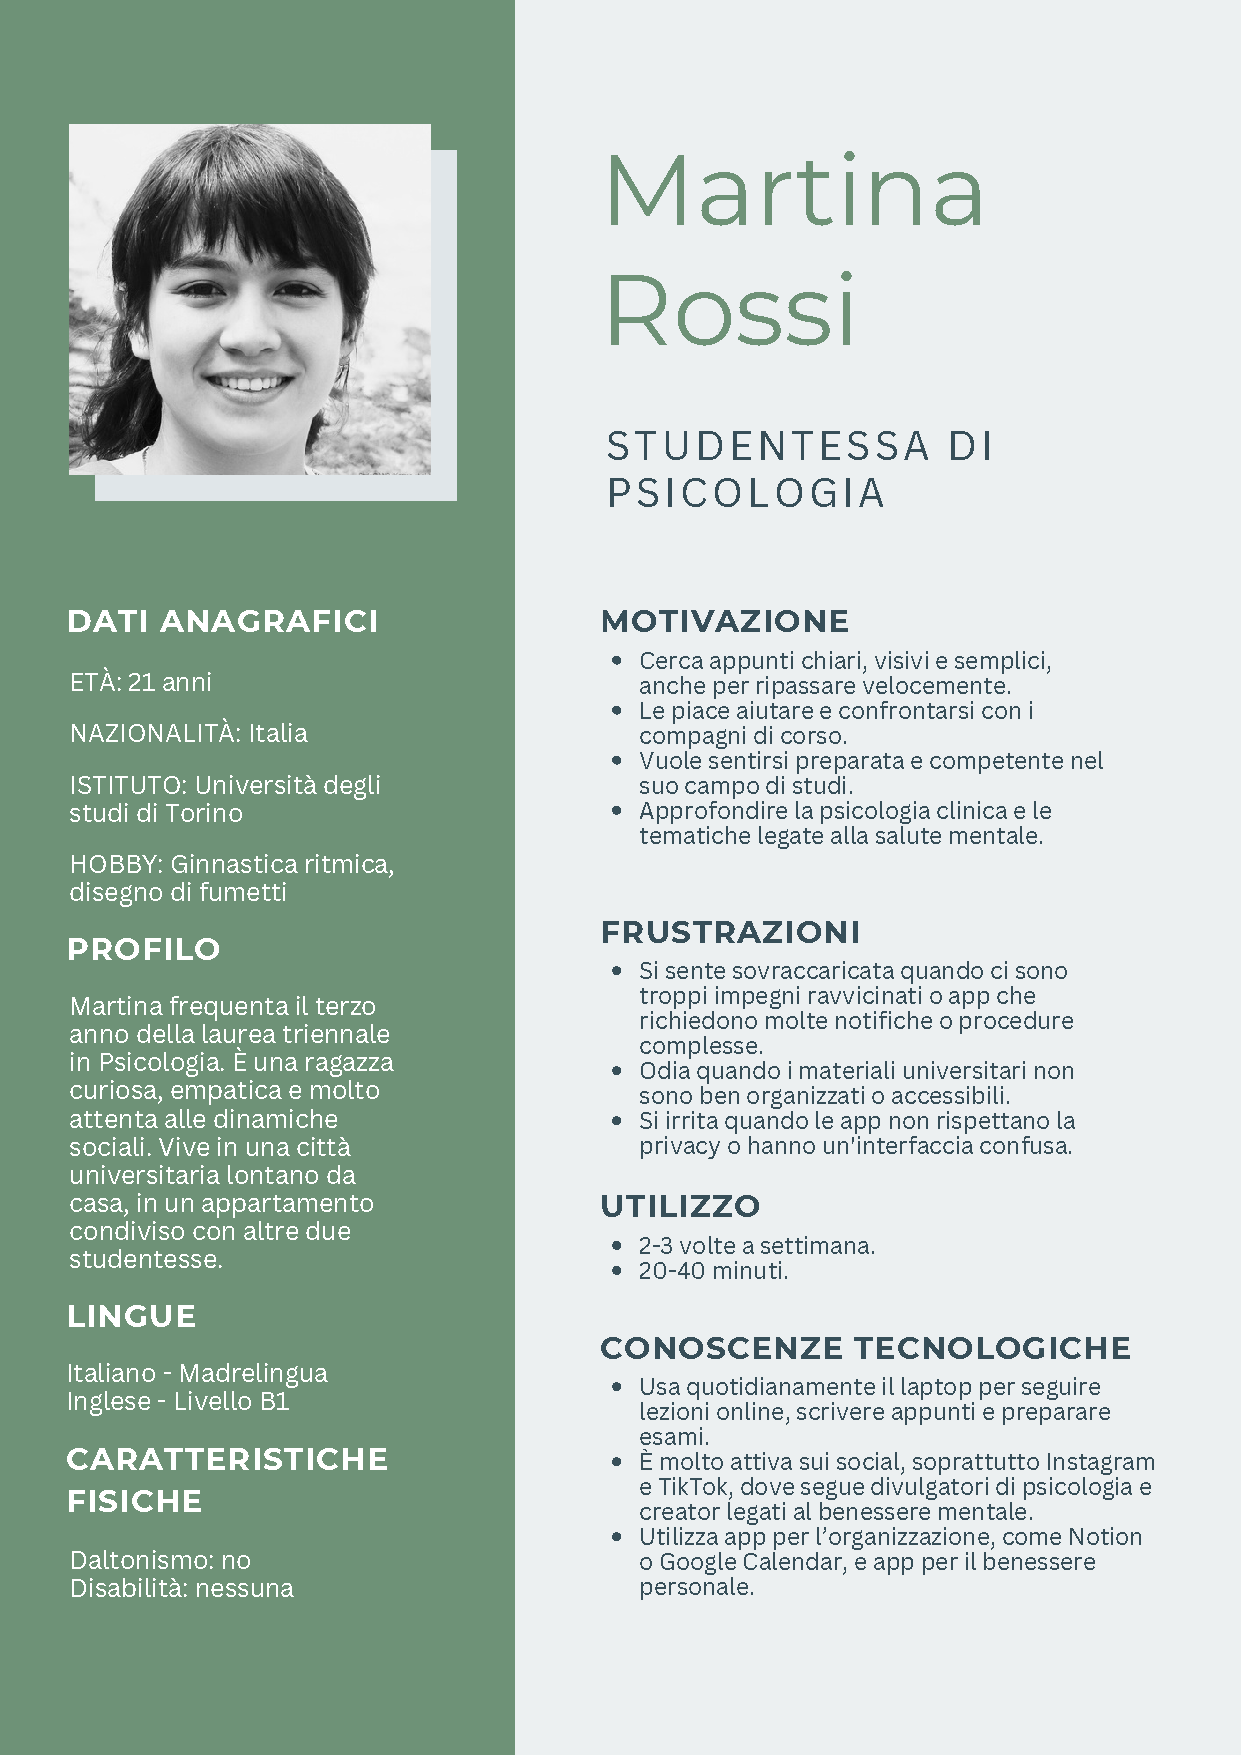
\includegraphics[width=0.67 \textwidth]{figures/02-profilo-utente/persona1.pdf}
  \caption{}
  \label{fig:2-1}
\end{figure}

\begin{figure}[h]
  \centering
  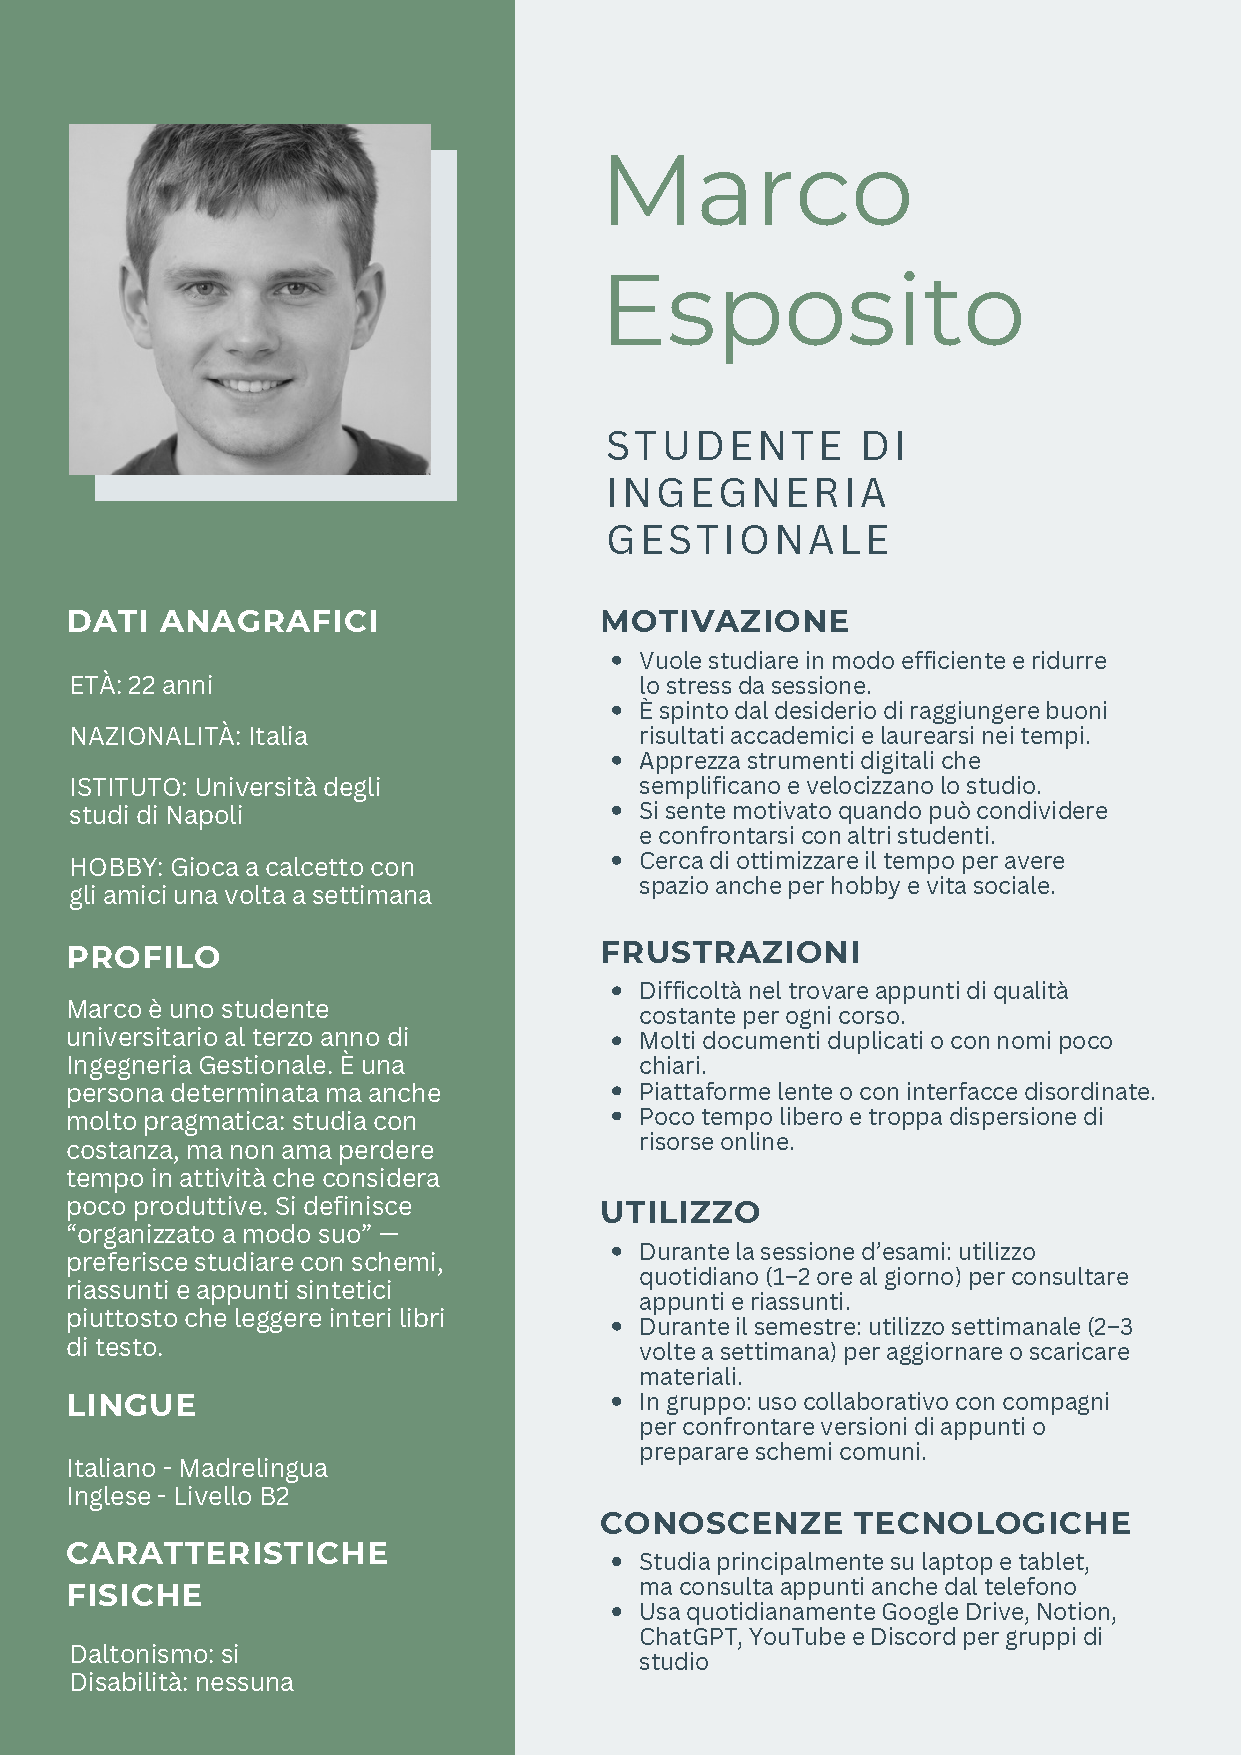
\includegraphics[width=0.67 \textwidth]{figures/02-profilo-utente/persona2.pdf}
  \caption{}
  \label{fig:2-2}
\end{figure}

\begin{figure}[h]
  \centering
  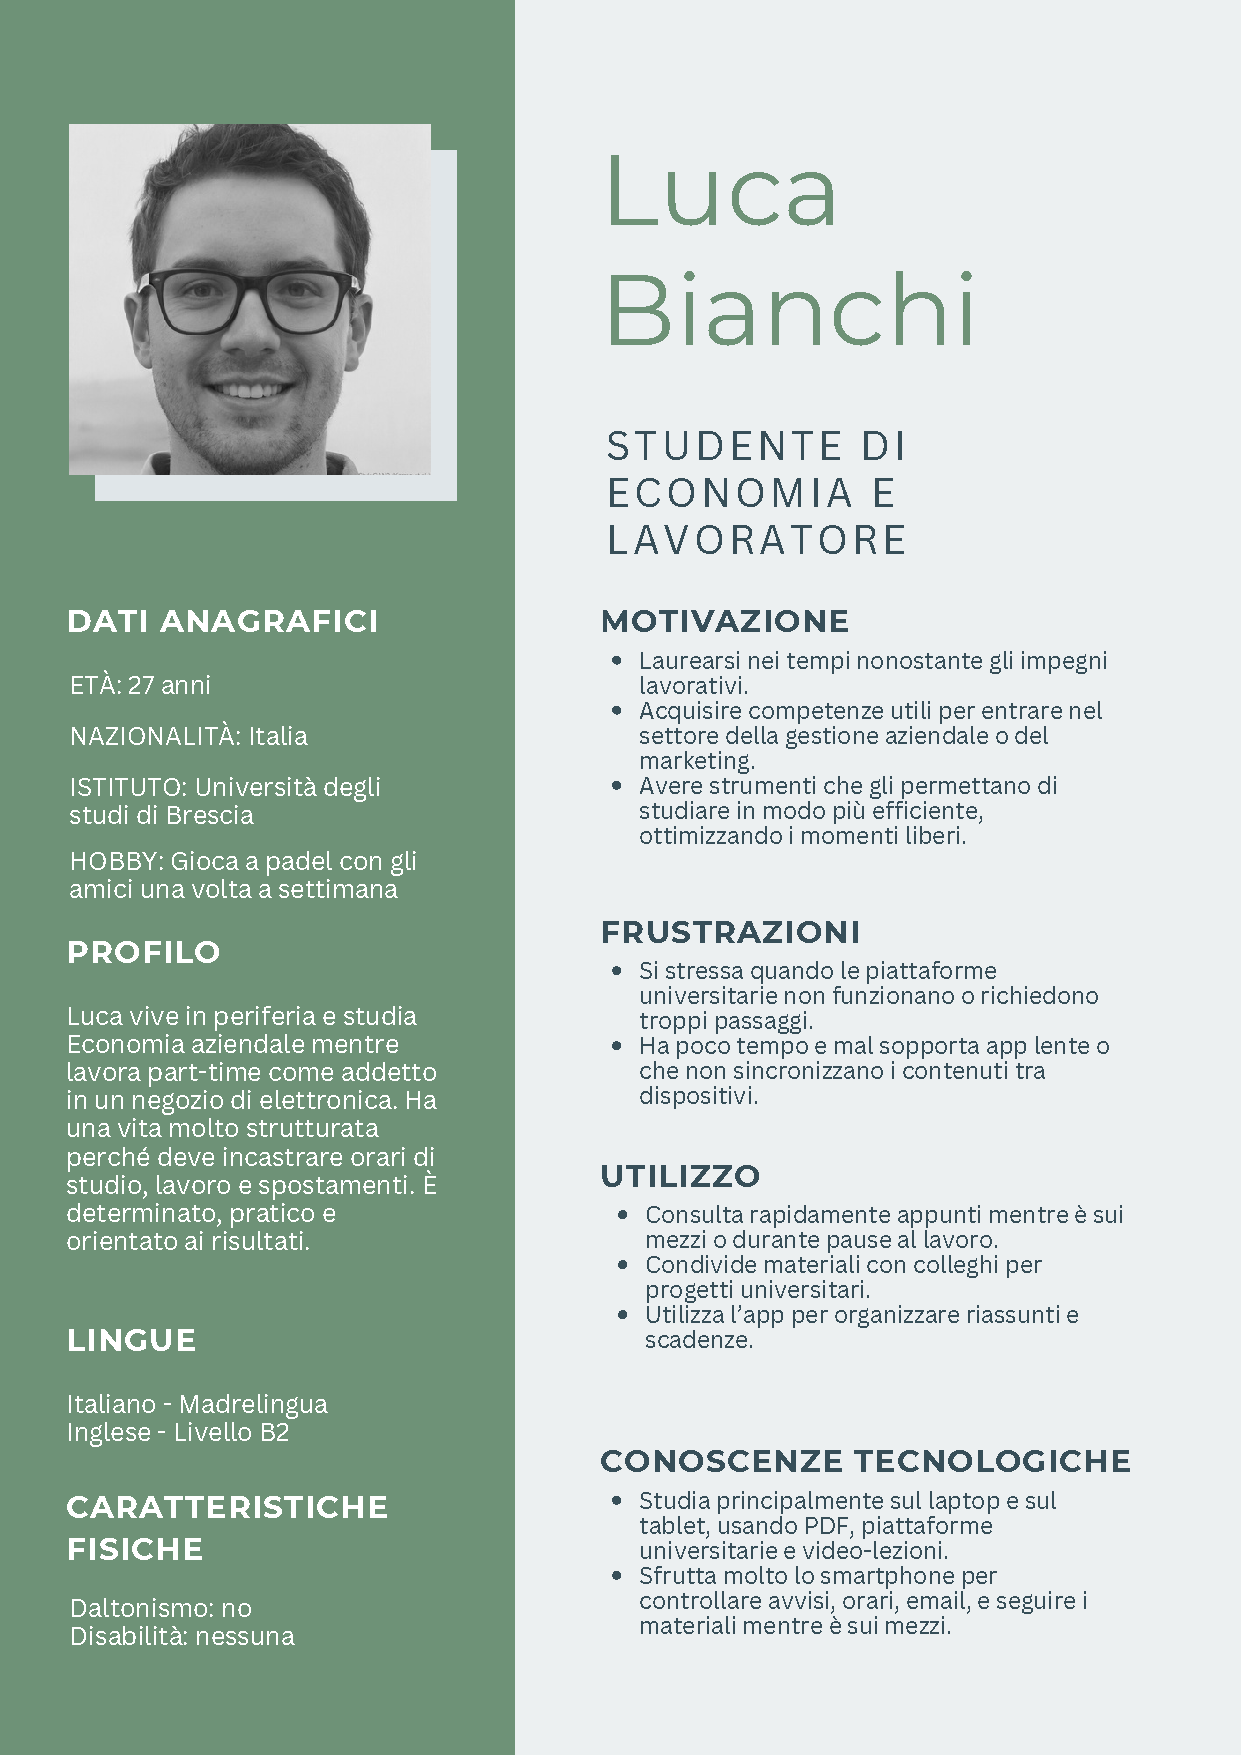
\includegraphics[width=0.67 \textwidth]{figures/02-profilo-utente/persona3.pdf}
  \caption{}
  \label{fig:2-3}
\end{figure}

\begin{figure}[h]
  \centering
  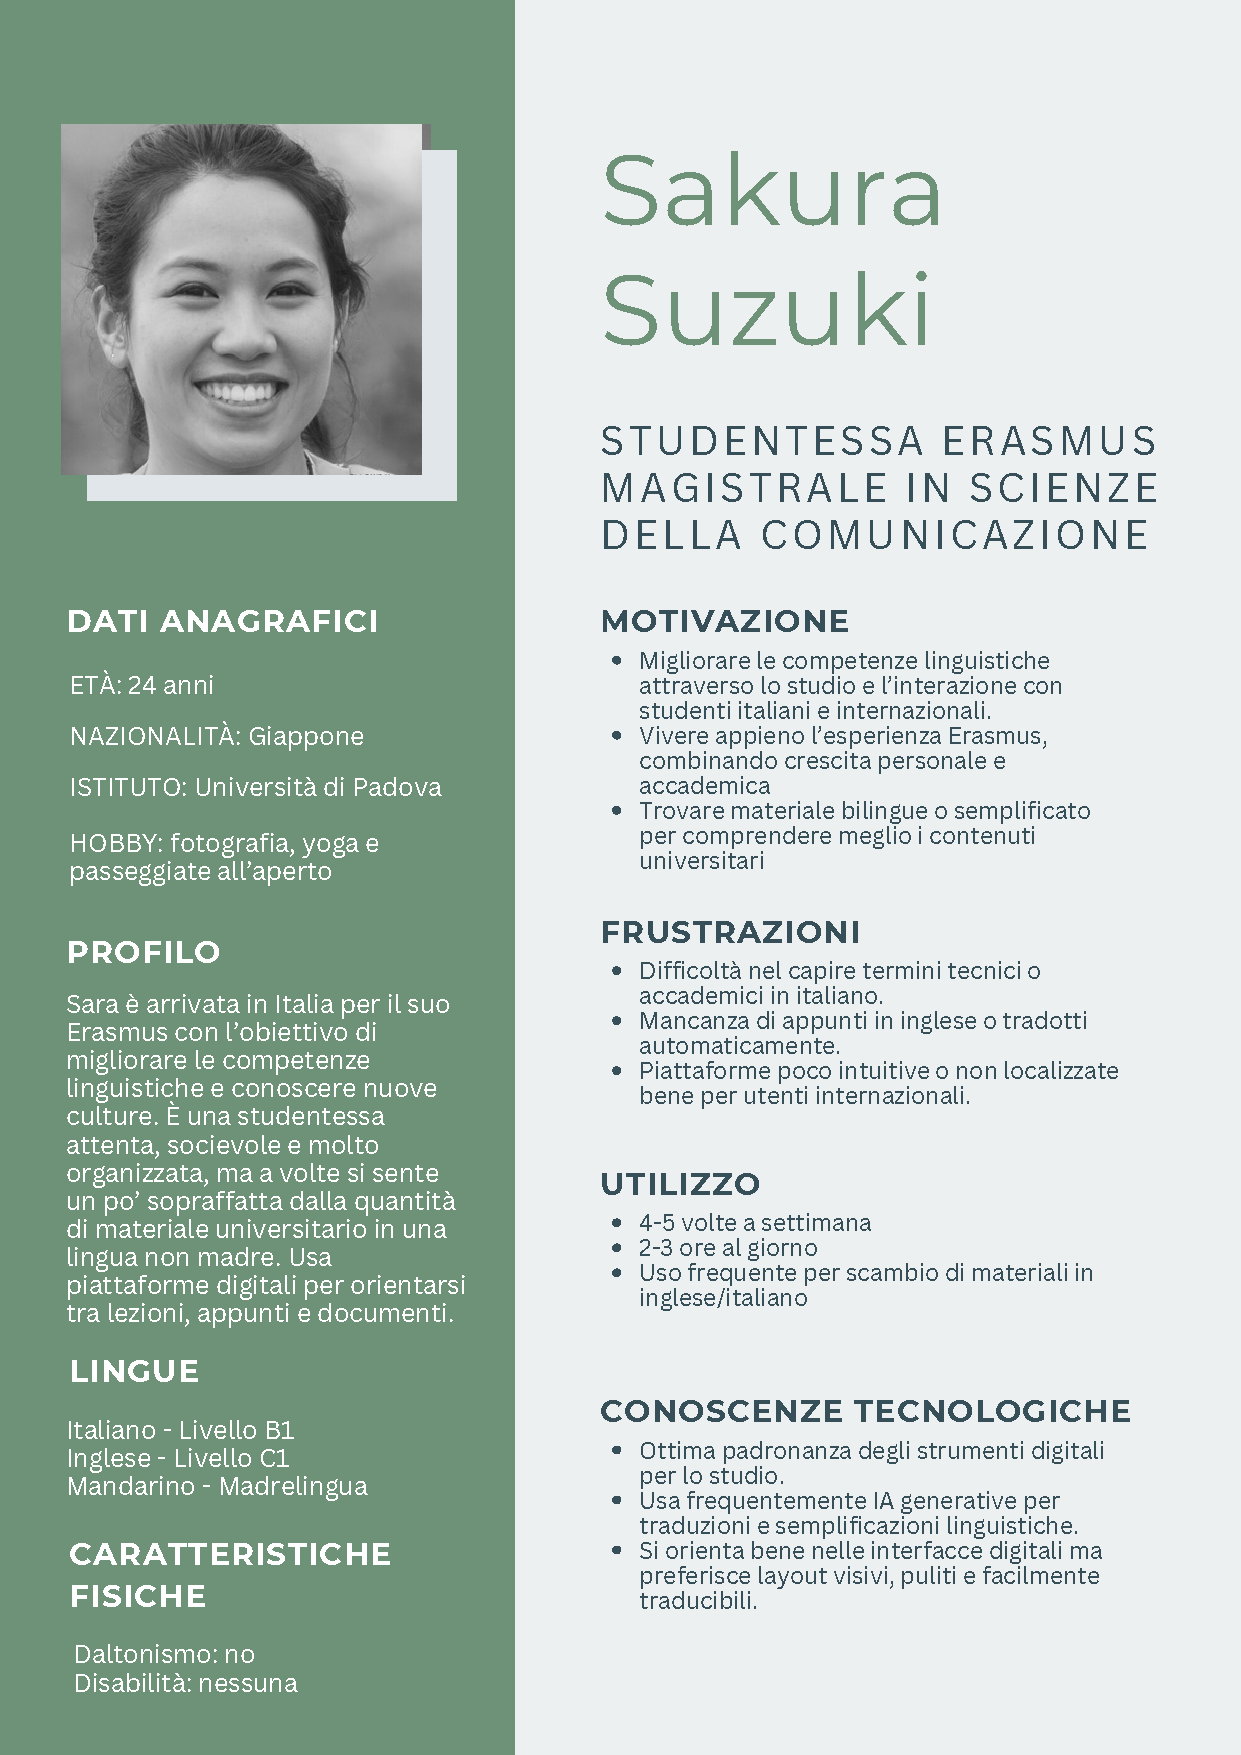
\includegraphics[width=0.67 \textwidth]{figures/02-profilo-utente/persona4.pdf}
  \caption{}
  \label{fig:2-4}
\end{figure}

\begin{figure}[h]
  \centering
  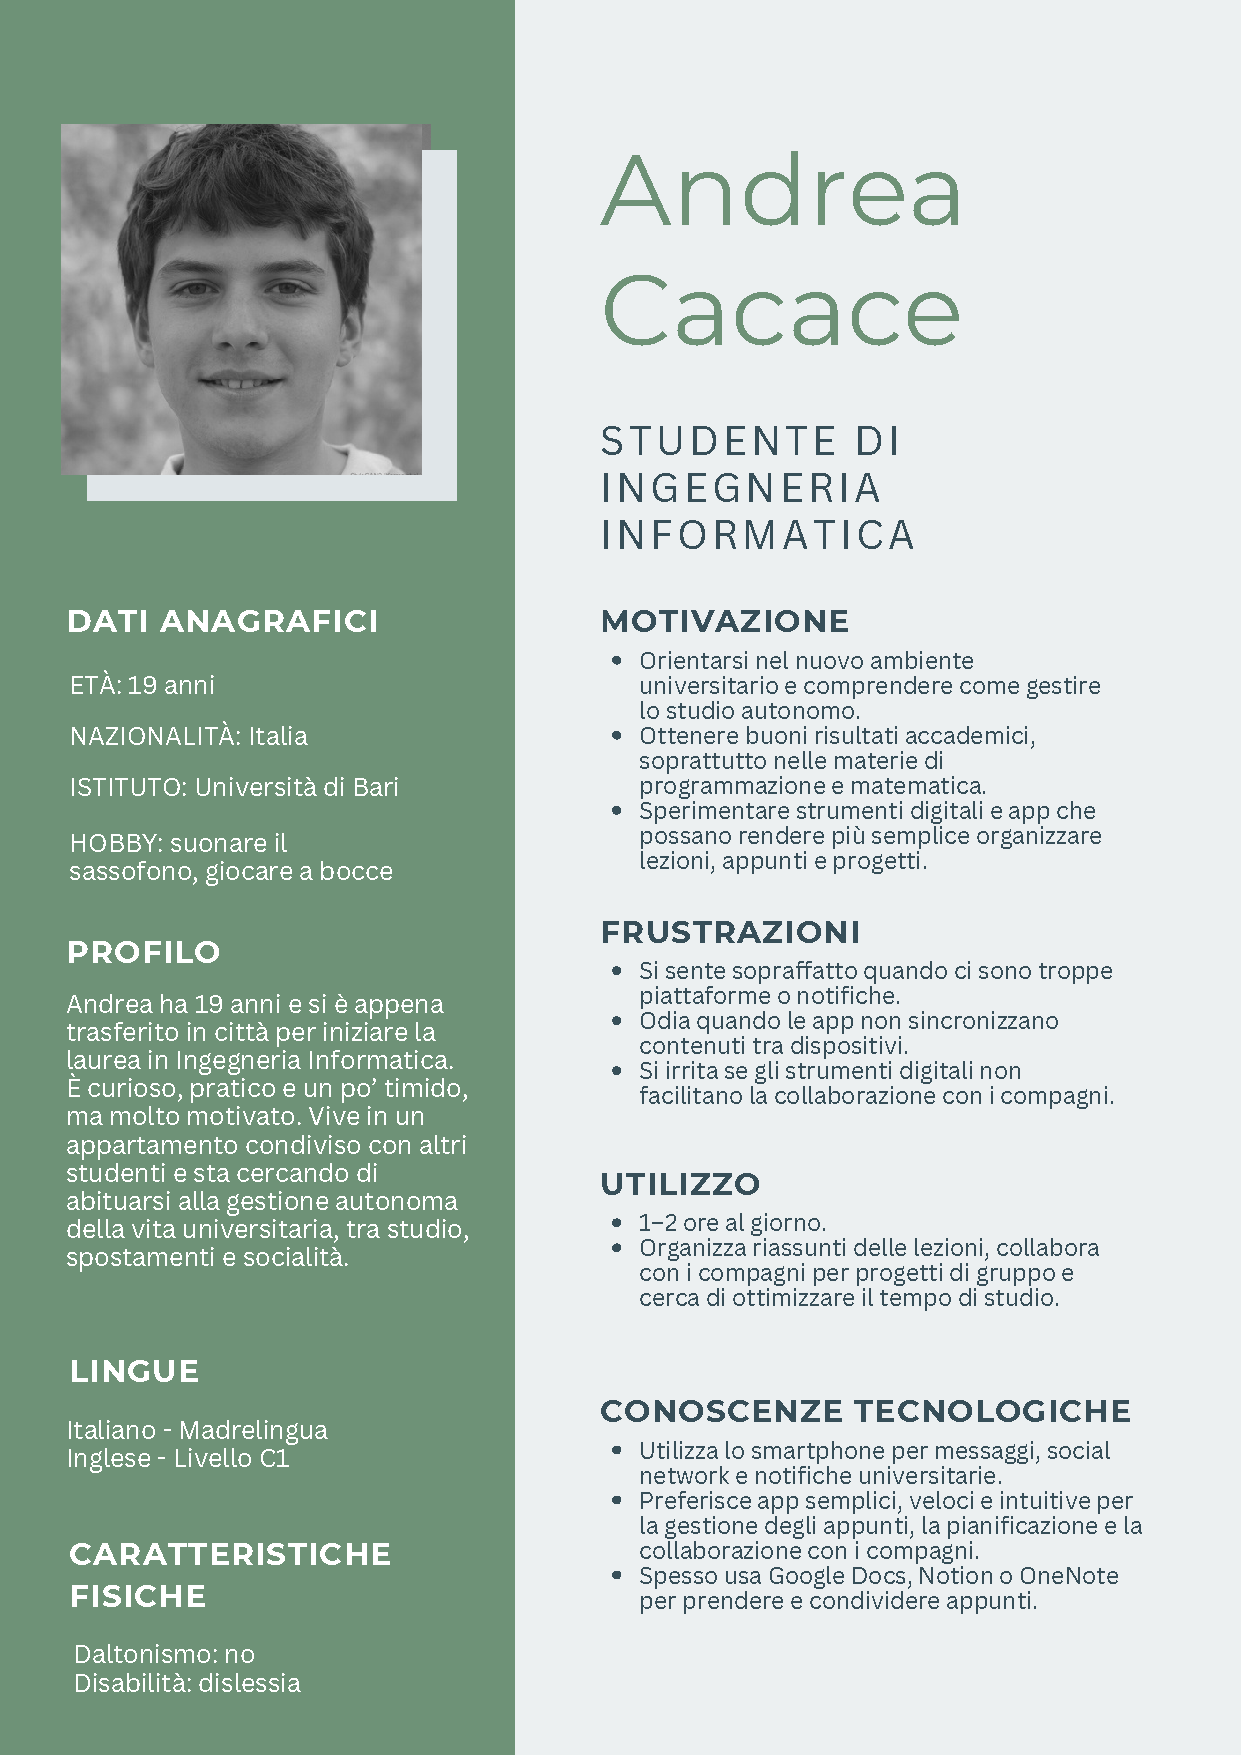
\includegraphics[width=0.67 \textwidth]{figures/02-profilo-utente/persona5.pdf}
  \caption{}
  \label{fig:2-5}
\end{figure}
